\chapter{Differentiation}


\section{Average Rate of Change}
We are all familiar with the concept of average speed. If you travel a distance of 120 km in 2 hours
then your average speed is 60 kph. There is a formula that you will have met 


\begin{center}
Average speed $ =\frac{\text{distance travelled}}{\text{time elapsed}}$
\end{center}\par
A distance/time graph can be drawn. 

The average speed can be expressed using
function notation 


\begin{center}
Average speed $ =\frac{s (b) -s (a)}{b -a}$
\end{center}\par
Finding the average rate of change is important in many contexts and in fact the average rate
of change can be defined for any function. 

The average rate of change of the function $y =f (x)$ is $\frac{\text{change in}y}{\text{change in}x}$ or $\frac{f (b) -f (a)}{b -a}$ 

The average rate of change is the slope of the \textbf{secant line} between $x =a$ and $x =b$ on the graph of $f$,\ that is the slope of the line that passes through $(a ,f (a))$ and $(b ,f (b))$. 

\subsection{Exercises 5.1}
\begin{enumerate}
\item Calculate the average rate of change for the function $f (x) =x^{2} +4$ between the following points 


\begin{enumerate}
\item $x =2$ and $x =6$ 

\item $x =5$ and $x =10$ 

\item $x =a$ and $x =a +h$ ($h \neq 0$) \end{enumerate}


\item [2.]
Calculate the average rate of change for the function $f (x) =3 x -5$ between the following points 


\begin{enumerate}
\item $x =0$ and $x =1$ 

\item $x =3$ and $x =7$ 

\item $x =a$ and $x =a +h$ ($h \neq 0$) 

\item Draw a conclusion from this. \end{enumerate}
\end{enumerate}


\section{Tangents, Velocities and Other Rates of Change}
We now investigate the process of changing the value of $(b -a)$ in the formula 

The average rate of change of the function
$y =f (x)$ is $\frac{\text{change in}y}{\text{change in}x}$ or $\frac{f (b) -f (a)}{b -a}$. 

As $(b -a)$ is made smaller and smaller the slope of the secant approaches the slope of the
tangent at $x =a$. The notation for this process is as follows. 

\subsection{Tangents}
\textbf{Definition:} The tangent line to the curve $y =f (x)$ at the point $P (a ,f (a))$ is the line through $P$ with slope $m =\underset{x \rightarrow a}{\lim }\frac{f (x) -f (a)}{x -a}$provided that limit exists. 

We sometimes refer to the slope of the tangent line to a curve at a point as the slope
of the curve at that point. The idea is that if we zoom in far enough towards the point then the curve looks
almost like a straight line. The more we zoom in the more the parabola looks like a straight line. 

Exercises 1 and 2 in section 3.1 give us a notation for the tangent line that is usually easier to use and is often preferred. 

Slope
of the secant line between $x =a$ and $x =a +h$ is $\frac{f (a +h) -f (a)}{h}$ 

Slope of the tangent line in the above definition becomes 


\begin{center}
$m =\underset{h \rightarrow 0}{\lim }\frac{f (a +h) -f (a)}{h}$
\end{center}\par


\subsection{Exercises 5.2.1}
\begin{enumerate}
\item Find the equation of the tangent line to the parabola $y =x^{2} +4$ at the point $(1 ,5)$. \end{enumerate}


\subsection{Velocities}
When this process is applied to the average velocity the result of computing the average velocity over shorter and shorter time intervals produces
the \textbf{instantaneous velocity}.\ Let $s =f (t)$ be the displacement at time $t$ then the \textbf{instantaneous velocity} is 


\begin{center}
$v (a) =\underset{h \rightarrow 0}{\lim }\frac{f (a +h) -f (a)}{h}$
\end{center}\par
This is often referred to as the \textbf{velocity at} $t =a$. 

\subsection{Other Rates of Change}
Suppose $y$ is a quantity that depend on another quantity $x$. Thus $y$ is a function of $x$ and we write $y =f (x)$. If we change from $x_{1}$ to $x_{2}$ then the change in $x$ is called an increment in $x$ and is denoted by 


\begin{center}
$ \Delta x =x_{2} -x_{1}$
\end{center}\par
and the corresponding increment in y is denoted by 


\begin{center}
$ \Delta y =y_{2} -y_{1}$
\end{center}\par
The average rate of change of $y$ with respect to $x$ over the interval $\left [x_{1} ,x_{2}\right ]$ is denoted by 


\begin{center}
$\frac{ \Delta y}{ \Delta x} =\frac{f (x_{2}) -f (x_{1})}{x_{2} -x_{1}}$
\end{center}\par
and can be interpreted geometrically as the slope of the secant line. As
we did with velocities we can compute the average rate of change over smaller and smaller intervals by letting $x_{2}$ approach $x_{1}$ and therefore letting $ \Delta x$ approach $0$. The limit of this process is called the instantaneous rate of change of $y$ with respect to $x$ at $x =x_{1}$. This is interpreted geometrically as the slope of the tangent to
the curve $y =f (x)$ at $(x_{1} ,f (x_{1}))$. 


\begin{center}
Instantaneous rate of change $ =\underset{ \Delta x \rightarrow 0}{\lim }\frac{ \Delta y}{ \Delta x} =\underset{x_{2} \rightarrow x_{1}}{\lim }\frac{f (x_{2}) -f (x_{1})}{x_{2} -x_{1}}$
\end{center}\par


\section{Derivatives}
Because the expression $\underset{h \rightarrow 0}{\lim }\frac{f (a +h) -f (a)}{h}$ occurs so widely it is given a special name and notation. 

The \textbf{derivative} of a function at a number
$a$, denoted by $f^{ \prime } (a)$ is 


\begin{center}
$f^{ \prime } (a) =\underset{h \rightarrow 0}{\lim }\frac{f (a +h) -f (a)}{h}$
\end{center}\par


\subsection{Exercises 5.3}
\begin{enumerate}
\item Find the derivative of the function $f (x) =5 x^{2} +3 x -1$ at the number $2$. 

\item Find the derivative of the function $f (x) =1 -3 x^{2}$ at the number $2$. 

\item Find the derivative of the function $f (x) =x^{4}$ at the number $1$, given
\begin{equation*}(x +h)^{4} =x^{4} +4 x^{3} h +6 x^{2} h^{2} +4 x h^{3} +h^{4}
\end{equation*}

\item Find the derivative of the function $F (x) =\sqrt{x}$ at the number $4$ Hint: rationalise the numerator \end{enumerate}


The process of finding the derivative using $f^{ \prime } (a) =\underset{h \rightarrow 0}{\lim }\frac{f (a +h) -f (a)}{h}\text{,}$ without using a formula that gives a short-cut to the answer, is called finding the derivative \textbf{from first principles}.


\section{The Derivative as a Function (The Derived Function)}
So far we have found a derivative of a function $f$ at a fixed number $a$ 


\begin{center}
\ $f^{ \prime } (a) =\underset{h \rightarrow 0}{\lim }\frac{f (a +h) -f (a)}{h}$
\end{center}\par
Now we change our point of view and let the number $a$ vary. If we replace $a$ in this equation with a variable $x$ we obtain 


\begin{center}
$f^{ \prime } (x) =\underset{h \rightarrow 0}{\lim }\frac{f (x +h) -f (x)}{h}$
\end{center}\par
Given any number $x$ for which this limit exists. We assign to $x$ the number $f^{ \prime } \left (x\right )$. So we can regard $f^{ \prime }$ as a new function which we call the \textbf{derived function} or the \textbf{derivative
of }$x$. 

\subsection{Exercises 5.4}
For exercises $1$ to $4$ in section 3.3 above find the derived function from first principles. 

\subsubsection{Other Notation for the Derived Function}
Given the notation $y =f (x)$ for the function the following alternative notations for $f^{ \prime } \left (x\right )$ are common 


\begin{center}
$f^{ \prime } (x) =y^{ \prime } =\frac{d y}{d x} =\frac{d f}{d x} =\frac{d}{d x} f (x)$ also $ =D f (x) =D_{x} f (x)$
\end{center}\par
The symbols $D$ and $\frac{d}{d x}$ are called \textbf{differential operators.} 

\subsection{Worksheet on Sketching Derived Functions}
The graph of $f (x) =(x -1) (x +2) (x -3)$ is drawn below. On the same set of axes, sketch the graph of the derived function, $f^{ \prime } (x)$\vspace{0.5cm} 

   
\setlength\fboxrule{0.01in}\setlength\fboxsep{0.2in}\fcolorbox[HTML]{000000}{FFFFFF}{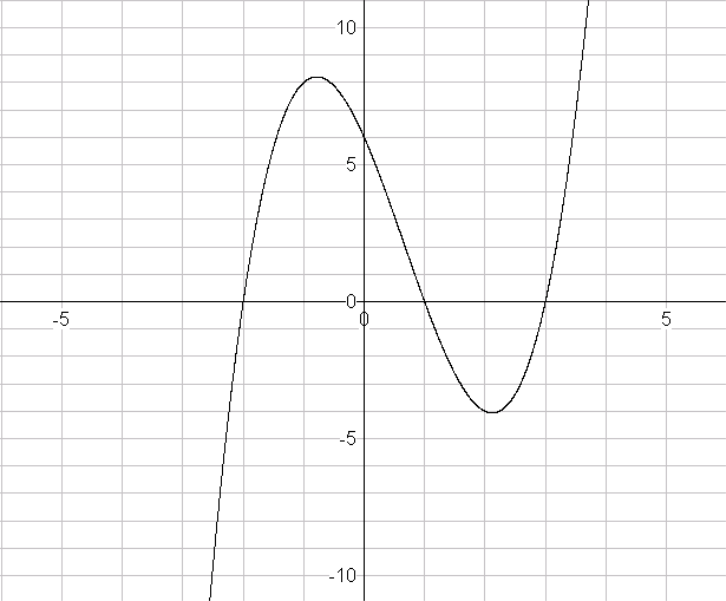
\includegraphics[ width=3.5526in, height=2.9473in,]{L4SZ2834}
}
\vspace{0.5cm} 

What is the shape of the graph of the derived function? 

The graph of $f (x) =(x +1) (x -1) (x -2) (x +3)$ is drawn below. On the same set of axes, sketch the graph of the derived function, $f^{ \prime } (x)\vspace{+0.500000cm}$ 

   
\setlength\fboxrule{0.01in}\setlength\fboxsep{0.2in}\fcolorbox[HTML]{000000}{FFFFFF}{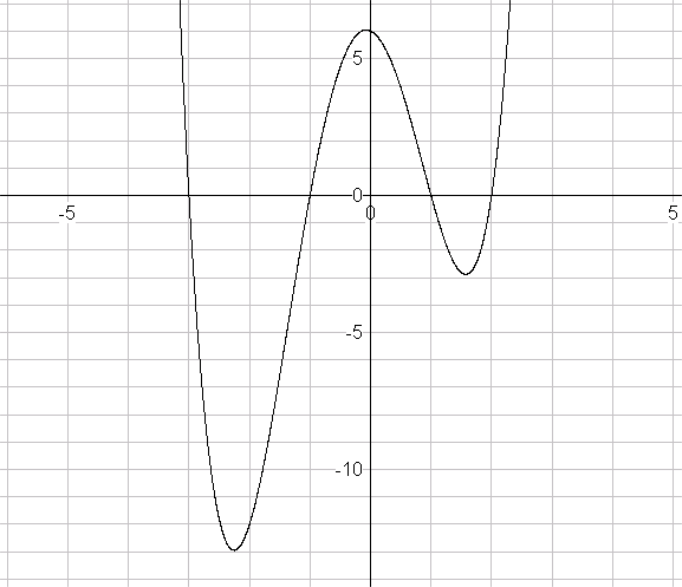
\includegraphics[ width=3.3633in, height=2.9014in,]{L4SZ2835}
}
\vspace{0.5cm}\vspace{0.5cm} 

What
is the order of $f (x)$? \vspace{0.5cm} 

What is the order of $f^{ \prime } (x)$?\vspace{0.5cm} 

 The
graph of $f (x) =e^{x}$ is drawn below. On the same set of axes, sketch the graph of the derived function, $f^{ \prime } (x)\vspace{+0.500000cm}$ 

   
\setlength\fboxrule{0.01in}\setlength\fboxsep{0.2in}\fcolorbox[HTML]{000000}{FFFFFF}{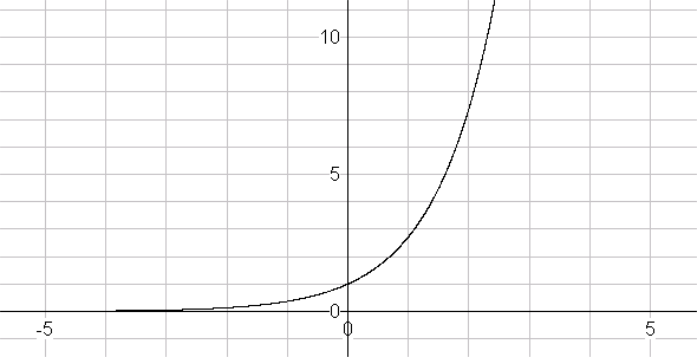
\includegraphics[ width=4.7167in, height=2.4275in,]{L4SZ2836}
}
\vspace{0.5cm} 

What is the shape of the graph of the derived function?\vspace{1cm}


The graph of $f (x) =10 x^{2} e^{x} (x +1)$is drawn below. On the same set of axes, sketch the graph of the derived function, $f^{ \prime } (x)\vspace{+0.500000cm}$ 

   
\setlength\fboxrule{0.01in}\setlength\fboxsep{0.2in}\fcolorbox[HTML]{000000}{FFFFFF}{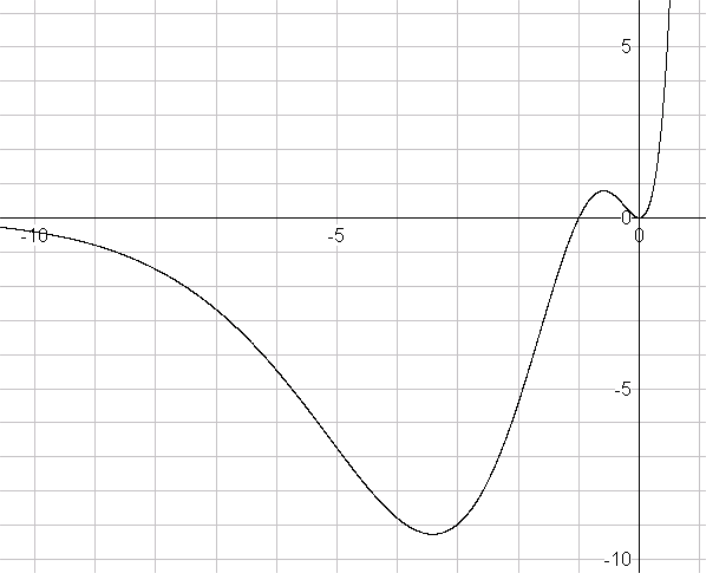
\includegraphics[ width=4.2851in, height=3.4826in,]{L4SZ2837}
}
 

\section{Derivatives of Polynomial Functions}
The constant function $f (x) =c$ 

The derivative can be found from first principles as follows: 


\begin{center}
$f^{ \prime } (x) =\underset{h \rightarrow 0}{\lim }\frac{f (x +h) -f (x)}{h} =\underset{h \rightarrow 0}{\lim }\frac{c -c}{h} =\underset{h \rightarrow 0}{\lim }0 =0$
\end{center}\par


\subsection{Power functions{\Large }${\Large f} ({\Large x}){\Large  =}{\Large x}^{n}$}
\bigskip When $f (x) =x$ it can be shown from first principles that $f^{ \prime } (x) =1$. Similarly when $f (x) =x^{2\text{}}$it can be shown that $f^{ \prime } (x) =2 x$ and when $f (x) =x^{3}$ it can be shown that $f^{ \prime } (x) =3 x^{2}$. 

As an example let us prove the formula for $f (x) =x^{4}$ from first principles
\begin{align*}f^{ \prime } (x) &  = \underset{h \rightarrow 0}{\lim }\frac{f (x +h) -f (x)}{h} \\
 &  = \underset{h \rightarrow 0}{\lim }\frac{(x +h)^{4} -x^{4}}{h} \\
 &  = \underset{h \rightarrow 0}{\lim }\frac{x^{4} +4 x^{3} h +6 x^{2} h^{2} +4 x h^{3} +h^{4} -x^{4}}{h} \\
 &  = \underset{h \rightarrow 0}{\lim }\frac{4 x^{3} h +6 x^{2} h^{2} +4 x h^{3} +h^{4}}{h} \\
 &  = \underset{h \rightarrow 0}{\lim }(4 x^{3} +6 x^{2} h +4 x h^{2} +h^{3}) \\
 &  = 4 x^{3}\end{align*}

This pattern is usually remembered in the following
form: If $f (x) =x^{n}$ then $f^{ \prime } (x) =n x^{n -1}$. 

Or alternatively $\frac{d}{d x} (x^{n}) =n x^{n -1}$. 

This pattern implies that $n$ must be a positive integer. 

It can be shown that from the definition of a derivative $\frac{d}{d x} \genfrac{(}{)}{}{}{1}{x} = -\frac{1}{x^{2}}$ or $y =x^{ -1}$ then $\frac{d y}{d x} = -1 \times x^{ -2}$, which proves the power rule for $n = -1$. 

Similarly if the exponent is a fraction it can be shown that the power rule holds 

e.g.
if $f (x) =\sqrt{x}$ then $f^{ \prime } (x) =\frac{1}{2 \sqrt{x}}$ or $f (x) =x^{\frac{1}{2}}$ then $f^{ \prime } (x) =\frac{1}{2} x^{ -\frac{1}{2}}$. 

It can be shown that the power rule holds for any real number $n$. 

\subsection{Exercises 5.5.1}
\begin{enumerate}
\item Differentiate 


\begin{enumerate}
\item $f (x) =\frac{1}{x^{2}}$ 

\item $y =\sqrt[{3}]{x^{2}}$ \end{enumerate}


\item Find the equations of the
tangent line and the normal line to the curve $y =x \sqrt{x}$ at the point $(1 ,1)$. \end{enumerate}


\subsubsection{Supplementary Exercises}
Differentiate the following expressions for $y$ with respect to $x$.  
%TCIMACRO{\TeXButton{Start 2 Cols}{\columnsep =30pt
% \begin {multicols}{2}}}%
%BeginExpansion
\columnsep =30pt
\begin {multicols}{2}
%EndExpansion
 


\begin{enumerate}
\item $y =x^{5}$ 

\item $y =\frac{1}{x^{3}}$ 

\item $y =x^{ -4}$ 

\item $y =x^{3/4}$ 

\item $y =\frac{1}{\sqrt{x}}$ \end{enumerate}



%TCIMACRO{\TeXButton{Stop 2 Cols}{\end {multicols}}}%
%BeginExpansion
\end {multicols}
%EndExpansion


\subsection{The Constant Multiple Rule}
If $c$ is a constant and $f$ is a differentiable function then 


\begin{center}
$\frac{d}{d x} \left [c f (x)\right ] =c \frac{d}{d x} f (x)$
\end{center}\par


\subsection{Exercises 5.5.2}
\begin{enumerate}
\item Differentiate 


\begin{enumerate}
\item $3 x^{4}$ 

\item $ -x$ \end{enumerate}
\end{enumerate}


\subsection{The Sum Rule}
If $f$ and $g$ are both differentiable then 


\begin{center}
$\frac{d}{d x} \left [f (x) +g (x)\right ] =\frac{d}{d x} f (x) +\frac{d}{d x} g (x)$
\end{center}\par


\subsection{The Difference Rule}
If $f$ and $g$ are both differentiable then 


\begin{center}
$\frac{d}{d x} \left [f (x) -g (x)\right ] =\frac{d}{d x} f (x) -\frac{d}{d x} g (x)$
\end{center}\par
These 3 rules are used together to allow us to differentiate any polynomial. 

\subsection{Exercises 5.5.3 and 5.5.4}
\begin{enumerate}
\item Differentiate $x^{8} +12 x^{5} -4 x^{4} +10 x^{3} -6 x +5$ 

\item Find the points on the curve $y =x^{4} -6 x^{2} +4$ where the tangent line is horizontal. \end{enumerate}


\subsubsection{Supplementary Exercises}
\columnsep=30pt
\begin{multicols}{2}

\begin{enumerate}
\item Differentiate 


\begin{enumerate}
\item $y =\frac{2}{5} x^{5}$ 

\item $y = -10$ 

\item $y = -3 x^{4}$ 

\item $y =\frac{2}{x^{4}}$ 

\item $y =\frac{1}{3 x^{3}}$ \end{enumerate}


\item Differentiate 


\begin{enumerate}
\item $f (t) =\sqrt{t}$ 

\item $f (t) =\sqrt{t^{3}}$ 

\item $f (z) =\sqrt[{3}]{z^{5}}$ 

\item $f (x) =2 x^{3.2}$ \end{enumerate}


\item Differentiate 


\begin{enumerate}
\item $f (x) =2 x^{3} -3 x^{2} +4 x -1$ 

\item $f (x) =x^{2} +x +1 +\frac{1}{x}$ \end{enumerate}


\item Given $s =4 t^{2} -7 t +5$ find $\frac{d s}{d t}$ 

\item Find $\frac{d \left (3 x\right )}{d x}$ 

\item Find $\frac{d \left (3 u^{4}\right )}{d u}$ 

\item Given $f (x) =2 x -3$ find $D f (x)$ \end{enumerate}
\end{multicols}

%\subsection{Graphing Lab}
%
%
%\subsubsection{To investigate the relationship between polynomial functions and their derived functions}
%\begin{description}
%\item [(a)] On the same grid draw the graph of $y =x^{2} -1$ and its derived function. \end{description}
%
%Look at where the derived function
%cuts the x-axis. Describe how this relates to the original curve.\vspace{2cm}
%
%
%Look at where the original function has a positive slope. Describe how this relates to
%the derived function.\vspace{2cm} 
%
%Look at where the original function has a negative
%slope. Describe how this relates to the derived function.\vspace{2cm}
%
%
%
%\begin{description}
%\item [(b)] On a \emph{new} grid draw the graph of $y =x (x +3) (x -3)$. Expand the brackets then differentiate and draw the graph of the derived function on the
%same grid. \end{description}
%
%What are the values of $x$ where the derived function cuts the $x$-axis? What does this tell you about the original function?\vspace{2cm}
%
%
%Zoom in to the local maximum point for the original curve and write down its coordinates.\vspace{2cm}
%
%
%Zoom in on the local minimum point for the original curve and write down its coordinates.\vspace{2cm}
%
%
%Write down the interval where the derived function is negative.\vspace{2cm} 
%
%Write down the interval where the original function is decreasing.\vspace{2cm} 
%
%Write
%down the intervals where the derived function is positive.\vspace{2cm} 
%
%Write down
%the intervals where the original function is increasing.\vspace{2cm} 
%
%Summarise your
%findings and indicate whether you believe this will always be the case.\vspace{2cm} 
%
%
%\begin{description}
%\item [(c)] To verify your findings in (b) above repeat the same steps with
%the polynomial function  \\\relax $y =x^{3} +4 x^{2} +x -6$ \end{description}
%
%\bigskip Coordinates of the maximum
%point are 
%
%\bigskip Coordinates of the minimum point are 
%
%\bigskip Interval
%where the derived function is negative is 
%
%\bigskip Interval where the original function is decreasing 
%
%\bigskip Intervals where the derived function is positive are \ \ \ \ \ \ \ \ \ \ \ \ and
%
%
%\bigskip Intervals where the original function is increasing are \ \ \ \ \ \ \ \ \ \ and
%
%
%\bigskip Does this confirm your finding in (b)? 

\section{Derivatives of Exponential Functions}
Let us try to compute the derivative of the exponential function $f (x) =a^{x}$ from first principles.
\begin{align*}f^{ \prime } (x) &  = \underset{h \rightarrow 0}{\lim }\frac{f (x +h) -f (x)}{h} =\underset{h \rightarrow 0}{\lim }\frac{a^{x +h} -a^{x}}{h} \\
 &  = \underset{h \rightarrow 0}{\lim }\frac{a^{x} a^{h} -a^{x}}{h} =\underset{h \rightarrow 0}{\lim }\frac{a^{x} \left (a^{h} -1\right )}{h} \\
\, &  &  \\
f^{ \prime } (x) &  = a^{x} \underset{h \rightarrow 0}{\lim }\frac{a^{h} -1}{h}\end{align*}

The factor $a^{x}$ doesn't depend on $h$, so can be taken in front of the limit
\begin{equation*}f^{ \prime } (x) =a^{x} \underset{h \rightarrow 0}{\lim }\frac{a^{h} -1}{h}
\end{equation*}

This limit is the value of the derived function where $x =0$, that is
\begin{equation*}f^{ \prime } (0) =\underset{h \rightarrow 0}{\lim }\frac{a^{h} -1}{h}
\end{equation*}

This means that provided $f (x)$ is differentiable
\begin{equation*}f^{ \prime } (x) =f^{ \prime } (0) a^{x}
\end{equation*}

This states that the rate of change of an exponential function is proportional to the function itself.


%\subsection{5.6.1 Excel lab on Exponential Functions}
%
%
%\subsubsection{To explore the value of $f^{ \prime } (0) =\underset{h \rightarrow 0}{\lim }\frac{a^{h} -1}{h}$for different values of $a$. and to derive the definition for $e$ as the value of $a$ that makes $\;\underset{h \rightarrow 0}{\lim }\frac{a^{h} -1}{h} =1$ i.e. $\underset{h \rightarrow 0}{\lim }\frac{e^{h} -1}{h} =1$}
%The value of $f^{ \prime } (0)$ is the slope of the tangent to the curve $f (x) =a^{x}$ where $x =0$ 
%
%
%\begin{description}
%\item [(a)] We will use Excel to produce a table of values where $h$ approaches $0$. \end{description}
%
%Firstly let $a =2$. Compute the value of $\frac{2^{h} -1}{h}$ as $h$ takes smaller and smaller values. 
%
%
%\begin{tabular}[c]{|l|l|}\hline
%$h$  & $\frac{2^{h} -1}{h}$  \\
%\hline
%$0.1$  &  \\
%\hline
%$0.01$  &  \\
%\hline
%$0.001$  &  \\
%\hline
%$0.0001$  &  \\
%\hline
%etc.
%&  \\
%\hline
%\end{tabular}\ You
%should show that $\frac{2^{h} -1}{h} \longrightarrow 0.693147$ as $h \longrightarrow 0$ 
%
%
%\begin{description}
%\item [(b)] Repeat with $a =3$ to show that $\frac{3^{h} -1}{h} \longrightarrow 1.098612$ as $h \longrightarrow 0$ \end{description}
%
%This shows that the slope of the tangent to $f (x) =2^{x}$ where $x =0$ is $0.693147$ and the slope of the tangent to $f (x) =3^{x}$ where $x =0$ is $1.098612$ 
%
%\bigskip
%\begin{description}
%\item [(c)] The number $e$ is the value of $a$ that gives the slope of the tangent where $x =0$ as $1$ \end{description}
%
%i.e. $f (x) =e^{x}$ and $f^{ \prime } (0) =1$. Devise a strategy to find the value of $e$ knowing that the slope of the tangent to $f (x) =2^{x}$ where $x =0$ is $0.693147$ and the slope of the tangent to $f (x) =3^{x}$ where $x =0$ is $1.098612$. 
%
%\bigskip 

\subsection{The Definition of $e$}
$e$ is the number such that $\underset{h \rightarrow 0}{\lim }\frac{e^{h} -1}{h} =1$ 

The Derivative of the Natural Exponential Function
\begin{equation*}\frac{d}{d x} \left (e^{x}\right ) =e^{x}
\end{equation*}

\textbf{Proof:} Previously we established that for $f (x) =a^{x}$ then $f^{ \prime } (x) =a^{x} \underset{h \rightarrow 0}{\lim }\frac{a^{h} -1}{h}$. Now we have shown that when $a =e$ we can put $\underset{h \rightarrow 0}{\lim }\frac{a^{h} -1}{h} =\underset{h \rightarrow 0}{\lim }\frac{e^{h} -1}{h} =1$ 

So $f (x) =e^{x}$ and $f^{ \prime } (x) =e^{x} \times 1 =e^{x}$. 

\bigskip The natural exponential function is unique in that it had the property that
it is its own derivative. Geometrically this means that the slope of the tangent at any point is the same as
the y-coordinate of that point. 

\subsection{Exercises 5.6.2}
\begin{enumerate}
\item Given $f (x) =e^{x} -x$ find $f^{ \prime } (x)$. Sketch the graph. 

\item A
what point on the curve $y =e^{x}$ is the tangent line parallel to the line $y =2 x$? \end{enumerate}


\subsubsection{Supplementary Exercises}
\begin{enumerate}
\item Find a point $a$ on the curve $f (x) =x^{3} +2 x^{2} +3 x +4$ where $f^{ \prime } (a) =2$. 

\item Differentiate $f (x) =\left (3 x\right )^{3}$. 

\item Differentiate $g (x) =\left (x^{3}\right )^{5}$ 

\item Find the derivative of $f (x) =e^{x} -x^{e}$. 

\item Find where the tangent line to the function $f (x) =x^{3} -x +1$ is parallel to the line $y =x$. 

\item Differentiate $f (x) =\frac{1}{x^{3}} -\frac{1}{\sqrt[{4}]{x^{3}}}$. 

\item Differentiate $f (x) =\frac{\sqrt{x} +\sqrt[{3}]{x}}{\sqrt[{4}]{x}}$. 

\item Find the derived function of $g (x) =e x^{2} +2 e^{x} +x e^{2} +x^{e^{2}}$ 

\item Find the derivative of $f (x) =\sqrt[{3}]{x} +\sqrt[{5}]{2}$. \end{enumerate}


\section{The Product and Quotient Rules}


\subsection{The Product Rule}
Let $f (x) =x$ and $g (x) =x^{2}$. What is the derivative of $f (x) \times g (x)$? The question helps to show that the answer is NOT $f^{ \prime } (x) \times g^{ \prime } (x)$ 

$f (x) \times g (x) =x \times x^{2} =x^{3}$ and we know the derivative of $x^{3}$ is $3 x^{2}$. Also we know that $f^{ \prime } (x) =1$ and $g^{ \prime } (x) =2 x$ so $f^{ \prime } (x) \times g^{ \prime } (x) =1 \times 2 x =2 x$ not $3 x^{2}$. 

So the derivative of the product of two functions is not the product
of the derivatives of each function. 

In symbols this can be written 


\begin{center}
$\left (f g\right )^{ \prime } \neq f^{ \prime } g^{ \prime }$
\end{center}\par
\textbf{Theorem} 

If $f$ and $g$ are both differentiable then $\frac{d}{d x} \left [f (x) g (x)\right ] =f (x) \frac{d}{d x} \left [g (x)\right ] +g (x) \frac{d}{d x} \left [f (x)\right ]$ 

\textbf{Proof} 

Let $u =f (x)$ and $v =g (x)$. If $x$ changes by an amount $ \Delta x$ then the corresponding changes in $u$ and $v$ are $ \Delta u =f (x + \Delta x) -f (x)\text{\quad \quad }$and$\text{\quad \quad } \Delta v =g (x + \Delta x) -g (x)$ 

The corresponding change in the product $u v$ is 


\begin{align*} \Delta (u v) &  = \left (u + \Delta u\right ) \left (v + \Delta v\right ) -u v \\
 &  = u v +u  \Delta v +v  \Delta u + \Delta u  \Delta v -u v \\
 &  = u  \Delta v +v  \Delta u + \Delta u  \Delta v\end{align*}

If we divide by $ \Delta x$, we get
\begin{equation*}\frac{ \Delta (u v)}{ \Delta x} =u \frac{ \Delta v}{ \Delta x} +v \frac{ \Delta u}{ \Delta x} + \Delta u \frac{ \Delta v}{ \Delta x}
\end{equation*}

Now we let $ \Delta x \rightarrow 0$
\begin{align*}\underset{}{\frac{d}{d x} \left (u v\right ) =\underset{ \Delta x \rightarrow 0}{\lim }} \genfrac{[}{]}{}{}{ \Delta (u v)}{ \Delta x} &  = \underset{ \Delta x \rightarrow 0}{\lim }\left [u \frac{ \Delta v}{ \Delta x}\right ] +\underset{}{\underset{ \Delta x \rightarrow 0}{\lim }\left [v \frac{ \Delta u}{ \Delta x}\right ]} +\underset{}{\underset{ \Delta x \rightarrow 0}{\lim }\left [ \Delta u \frac{ \Delta v}{ \Delta x}\right ]} \\
\frac{d}{d x} (u v) &  = u \frac{d v}{d x} +v \frac{d u}{d x} +0. \frac{d v}{d x}\end{align*}

So
\begin{equation*}\frac{d}{d x} \left [f (x) g (x)\right ] =f (x) \frac{d}{d x} \left [g (x)\right ] +g (x) \frac{d}{d x} \left [f (x)\right ]
\end{equation*}

The Product rule is often seen in an abbreviated form as
\begin{equation*}\left (u v\right )^{ \prime } =u v^{ \prime } +v u^{ \prime }
\end{equation*}

In words the Product Rule states that \textit{the derivative of the product of two functions is
the first function times the derivative of the second function plus the second function times the derivative of the first function.} 

\subsection{Exercises 5.7.1}
\begin{enumerate}
\item If $f (x) =x e^{x}$ find $f^{ \prime } (x)$. 

\item Find the derivative of $g (x) =x^{2} e^{x}$. 

\item If $y =\left (r^{2} -2 r\right ) e^{r}$ find $\frac{d y}{d r}$. \end{enumerate}


\subsubsection{Supplementary Exercises}
Differentiate with respect to $x$ 


\begin{enumerate}
\item $x^{3} e^{x}$ 

\item $x^{ -3} e^{x}$ 

\item $\left (x +1\right ) e^{x}$ 

\item $\left (x +2\right ) \left (x -2\right ) e^{x}$ \end{enumerate}


\subsection{The Quotient Rule}
Let $u =f (x)$ and $v =g (x)$ be differentiable functions of $x$ then we can show that
\begin{equation*}\frac{d}{d x} \genfrac{[}{]}{}{}{f (x)}{g (x)} =\frac{g (x) \frac{d}{d x} \left [f (x)\right ] -f (x) \frac{d}{d x} \left [g (x)\right ]}{\left [g (x)\right ]^{2}}
\end{equation*}or in abbreviated form
\begin{equation*}\genfrac{(}{)}{}{}{u}{v}^{ \prime } =\frac{v u^{ \prime } -u v^{ \prime }}{v^{2}}
\end{equation*}or in words \textit{the derivative of a quotient is the denominator times the derivative of the numerator minus the numerator
times the derivative of the denominator, all divided by the square of the denominator.}
\begin{align*} \Delta \genfrac{(}{)}{}{}{u}{v} &  = \frac{u + \Delta u}{v + \Delta v} -\frac{u}{v} =\frac{\left (u + \Delta u\right ) v -u \left (v + \Delta v\right )}{v \left (v + \Delta v\right )} \\
 &  = \frac{v  \Delta u -u  \Delta v}{v \left (v + \Delta v\right )}\end{align*}

If we divide by $ \Delta x$, we get
\begin{equation*}\frac{ \Delta \genfrac{(}{)}{}{}{u}{v}}{ \Delta x} =\frac{v \frac{ \Delta u}{ \Delta x} -u \frac{ \Delta v}{ \Delta x}}{v \left (v + \Delta v\right )}
\end{equation*}

So
\begin{equation*}\frac{d}{d x} \genfrac{(}{)}{}{}{u}{v} =\underset{ \Delta x \rightarrow 0}{\lim }\frac{ \Delta \genfrac{(}{)}{}{}{u}{v}}{ \Delta x} =\underset{ \Delta x \rightarrow 0}{\lim }\frac{v \frac{ \Delta u}{ \Delta x} -u \frac{ \Delta v}{ \Delta x}}{v \left (v + \Delta v\right )}
\end{equation*}

As $ \Delta x \rightarrow 0$, $ \Delta v \rightarrow 0$, $\frac{ \Delta u}{ \Delta x} \rightarrow \frac{d u}{d x}$ and $\frac{ \Delta v}{ \Delta x} \rightarrow \frac{d v}{d x}$ 

So
\begin{equation*}\frac{d}{d x} \genfrac{(}{)}{}{}{u}{v} \rightarrow \frac{v \frac{d u}{d x} -u \frac{d v}{d x}}{v^{2}}
\end{equation*}

\subsection{Exercises 5.7.2}
\begin{enumerate}
\item Given $y =\frac{3 x +1}{2 x -1}$ find $y^{ \prime }$. 

\item Differentiate $y =\frac{e^{x}}{x +1}$. 

\item If $f (t) =\frac{2 t}{1 +t^{2}}$ find $\frac{d f}{d t}$. 

\item Find the derived function for $f (x) =\frac{A}{B +C e^{x}}$. \end{enumerate}


\subsubsection{Supplementary Exercises}
Differentiate 


\begin{enumerate}
\item $\frac{3 x^{2}}{1 -x}$ 

\item $\frac{x}{x +2}$ 

\item $\frac{\sqrt{x}}{x +2}$ 

\item $\frac{2 x^{2} +3 x +2}{e^{x}}$ \end{enumerate}


\subsection{5.7.3 Exercises involving Tangent and Normals}
\begin{enumerate}
\item Find the equation of the tangent line and normal line to the curve $y =x e^{x}$ at the point $\left (0 ,0\right )$ 

\item The
curve $y =1/(1 +x^{2})$ has the name \textbf{witch of Maria Agnesi.} 


\begin{description}
\item [(a)] Find the equation of the tangent line to this curve at the point
$\left (1 ,\frac{1}{2}\right )$. 

\item [(b)]
Use Desmos to draw the graph of the curve and the tangent line on the same grid. \end{description}

\item The
curve $y =x/(1 +x^{2})$ is called a \textbf{serpentine}. 


\begin{description}
\item [(a)] Find the equation of the tangent line at the point $\left (1 ,\frac{1}{2}\right )$. 

\item [(b)]
Use Desmos to draw the graph of the curve and the tangent line on the same grid. \end{description}\end{enumerate}


\section{Differentiation of a Composite Function}


\subsection{Examples of Composite Functions}
Let $f (x) =x^{2}$ and $g (x) =2 x +1$ then $\left (f \circ g\right ) (x) =f \left (g \left (x\right )\right ) =f (2 x +1) =\left (2 x +1\right )^{2}$. 

Also $\left (g \circ f\right ) (x) =g \left (x^{2}\right ) =2 \left (x^{2}\right ) +1 =2 x^{2} +1$. 

\subsection{Exercises 5.8.1}
\begin{enumerate}
\item Let $f (x) =\sqrt{x}$ and $g (x) =x^{3}$ find $\left (f \circ g\right ) (x)$ and $\left (g \circ f\right ) \left (x\right )$. 

\item Given $h \left (x\right ) =e^{x}$ and $j (x) =\frac{x^{2}}{2}$ find $\left (h \circ j\right ) (x)$ and $\left (j \circ h\right ) (x)$. \end{enumerate}


\subsection{Recognising Composite Functions}
The differentiation rules we have met so far allow us to differentiate pairs of functions that have been added, subtracted, multiplied or divided.
\ They do not allow us to differentiate an expression that is made from a function that is within another function.


\subsubsection{Examples}
\begin{enumerate}
\item We can differentiate $x^{2}$ but we can't use the same procedure to differentiate $\left (1 -x\right )^{2}$. 

\item We can differentiate $\frac{1}{x^{2}}$ but we can't use the same procedure to differentiate $\frac{1}{x^{2} +1}$. 

\item We can differentiate e$^{x}$ but we can't use the same procedure to differentiate $e^{x^{2}}$. \end{enumerate}


These are examples of composite functions. 

For
example if $f (x) =x^{2}$ and $g (x) =1 -x$ then $\left (f \circ g\right ) (x) =f (1 -x) =\left (1 -x\right )^{2}$ 

A name often used for functions of this type is \emph{function of a function.} 

\subsection{The Chain Rule}
Once we recognise we are dealing with a composite function we need a procedure to differentiate it. You
will find that you are far more likely to be required to differentiate a composite function in a practical situation than a simple one. It
can be proved that the derivative of the composite function $f \circ g$ is the product of the derivatives of $f$ and $g$. This important rule is given the name the \emph{Chain Rule}.
\ A substitution method is often used to add clarity to the differentiation process. 

Let
$y =u^{2}$ and let $u =1 -x$. Then $\frac{d y}{d u} =2 u$ and $\frac{d u}{d x} = -1$. Now $\frac{d y}{d x} =\frac{d y}{d u} \cdot \frac{d u}{d x} =2 u \times ( -1) = -2 u = -2 (1 -x) =2 (x -1)$. 

The Leibniz form of the Chain Rule $\frac{d y}{d x} =\frac{d y}{d u} \frac{d u}{d x}$ is what gives the rule its name. Because of the apparent cancelling it is particularly
easy to learn in this form. 

As an aside let us verify the rule for this example. Given
$y =(1 -x)^{2}$. We will expand the right hand side of the equation. It
becomes $y =x^{2} -2 x +1$. So $y^{ \prime } =2 x -2 =2 (x -1)$ as before. 

Using function notation the Chain Rule states: If $f$ and $g$ are both differentiable and $F =f \circ g$ is the\ composite function $F (x) =f (g (x))$, then $F$ is differentiable and $F^{ \prime } =f^{ \prime } (g (x)) g^{ \prime } (x)$. 

The proof is not as straightforward as the others we have met so far so will not be covered in the course. 

To illustrate the difficulty let us proceed as we have done in the proofs of the product rule and quotient rule until we find a flaw in our reasoning.


Let $u =g (x)$ then if $x$ is given an increment of $ \Delta x$ the corresponding increment in $u$ is $ \Delta u$. So
\begin{equation*} \Delta u =g (x + \Delta x) -g (x)
\end{equation*}

And if $y =f (g (x))$ then $y =f (u)$ so the corresponding change in $y$ is
\begin{equation*} \Delta y =f (u + \Delta u) -f (u)
\end{equation*}

We can write
\begin{equation*}\frac{d y}{d x} =\underset{ \Delta x \rightarrow 0}{\lim }\frac{ \Delta y}{ \Delta x}
\end{equation*}

But we are not able to expand this to become
\begin{align*} &  = \underset{ \Delta x \rightarrow 0}{\lim }\frac{ \Delta y}{ \Delta u} \cdot \frac{ \Delta u}{ \Delta x} \\
 &  = \underset{ \Delta x \rightarrow 0}{\lim }\frac{ \Delta y}{ \Delta u} \cdot \underset{ \Delta x \rightarrow 0}{\lim } \frac{ \Delta u}{ \Delta x} \\
 &  = \underset{ \Delta u \rightarrow 0}{\lim }\frac{ \Delta y}{ \Delta u} \cdot \underset{ \Delta x \rightarrow 0}{\lim } \frac{ \Delta u}{ \Delta x} \\
 &  = \frac{d y}{d u} \cdot \frac{d u}{d x}\end{align*}

The reason we can't prove the rule in this way is that $ \Delta u$ could be equal to $0$ even when $ \Delta x \neq 0$ which would mean we are dividing by zero. However the procedure at least suggests
the chain rule is feasible. 

\subsection{A Comment on the Leibniz form of the Chain Rule}
$\frac{d y}{d x} =\frac{d y}{d u} \cdot \frac{d u}{d x}$ gives the impression that the $d u$ could cancel but remember we have not defined $d u$. We have defined $\frac{d y}{d u}$ as the rate of change of $y$ with respect to $u$ and $\frac{d u}{d x}$ as the rate of change of $u$ with respect to $x$. However the apparent cancelling helps us to remember the way the differentials
are arranged. it also helps us to accept the extension of the Chain Rule to cover a function of a function of
a function etc. e.g.
\begin{align*}\text{Let}y &  = f (u)\text{,}u =g (v)\text{and}v =h (x) \\
\text{Then}\frac{d y}{d x} &  = \frac{d y}{d u} \cdot \frac{d u}{d v} \cdot \frac{d v}{d x}\end{align*}

\textbf{Example} 

Find $F^{ \prime } (x)$ when $F (x) =\frac{1}{x^{2} +1}$. 

Using the function notation 

$F (x) =\left (f \circ g\right ) (x) =f (g (x))$ where $f (u) =u^{ -1}$ and $g (x) =x^{2} +1$
\begin{equation*}f^{ \prime } (u) = -u^{ -2}\text{and}g^{ \prime } (x) =2 x
\end{equation*}

and 


\begin{align*}F^{ \prime } (x) &  = f^{ \prime } (g (x)) g^{ \prime } (x) \\
 &  = \frac{ -1}{(x^{2} +1)^{2}} \cdot 2 x \\
 &  = \frac{ -2 x}{\left (x^{2} +1\right )^{2}}\end{align*}

Using the Leibniz notation 

Let $u =x^{2} +1$ and $y =u^{ -1}$ then
\begin{align*}F^{ \prime } (x) &  = \frac{d y}{d u} \frac{d u}{d x} = -u^{ -2} \left (2 x\right ) \\
 &  = \frac{ -1}{\left (x^{2} +1\right )^{2}} \left (2 x\right ) =\frac{ -2 x}{\left (x^{2} +1\right )^{2}}\end{align*}

To use the method we need to bring a new variable into the problem we are trying to solve. It
is recommended that you use the variable $u$ wherever possible so that you follow through using a pattern you are familiar with. 

\subsection{Formal Statement of the Chain Rule}
If $g$ is differentiable at $x$ and $f$ is differentiable at $g (x)$, then the composite function $F =f \circ g$ defined by $F (x) =f (g (x))$ is differentiable at $x$ and $F^{ \prime }$ is given by the product
\begin{equation*}F^{ \prime } (x) =f^{ \prime } (g (x)) \cdot g^{ \prime } (x)
\end{equation*}

In Leibniz notation, if $y =f (u)$ and $u =g (x)$ are both differentiable functions, then
\begin{equation*}\frac{d y}{d x} =\frac{d y}{d u} \cdot \frac{d u}{d x}
\end{equation*}

\subsection{Exercises 5.8.5}
\begin{enumerate}
\item   
%TCIMACRO{\TeXButton{Start 2 Cols}{\columnsep =30pt
% \begin {multicols}{2}}}%
%BeginExpansion
\columnsep =30pt
\begin {multicols}{2}
%EndExpansion
 Find $F^{ \prime } (x)$ when $F (x) =\sqrt{1 +x^{2}}$. 

\item Given $y =\left (1 -x^{2}\right )^{5}$ find $\frac{d y}{d x}$. 

\item Find the derivative of $e^{x^{2}}$. 

\item Find the derived function for $e^{e^{x}}$. 
%TCIMACRO{\TeXButton{Stop 2 Cols}{\end {multicols}}}%
%BeginExpansion
\end {multicols}
%EndExpansion
 \end{enumerate}


\subsubsection{Supplementary Exercises}
Differentiate with respect to $x$ 


\begin{enumerate}
\item   
%TCIMACRO{\TeXButton{Start 2 Cols}{\columnsep =30pt
% \begin {multicols}{2}}}%
%BeginExpansion
\columnsep =30pt
\begin {multicols}{2}
%EndExpansion
 $\left (3 x +2\right )^{3}$ 

\item $\left (4 -3 x\right )^{3}$ 

\item $\left (5 x +3\right )^{\frac{3}{5}}$ 

\item $\frac{1}{2 x +1}$ 

\item $\frac{3}{\left (4 -x\right )^{3}}$ 

\item $\sqrt{2 x -5}$ 

\item $\sqrt[{3}]{5 -x^{2}}$ 

\item $\frac{1}{\sqrt{x +2}}$ 

\item $e^{2 x^{3}}$ 
%TCIMACRO{\TeXButton{Stop 2 Cols}{\end {multicols}}}%
%BeginExpansion
\end {multicols}
%EndExpansion
 \end{enumerate}


\section{Combining the Chain Rule with the Product Rule}
The Chain Rule will be found in many situations where functions are added, subtracted, multiplied or divided. As
an example we will focus on combining the Chain Rule with the Product Rule, however any combination of these 5 rules could be found in a problem. 

\subsubsection{Example}
Differentiate $x e^{ -x^{2}}$. 

We can see that there is a product of two functions present in this example, i.e. $f (x) =x$ and $g (x) =e^{ -x^{2}}$. Also $g (x)$ is a composite function. 

We have from the Product Rule
\begin{equation*}\left (f g\right )^{ \prime } =f g^{ \prime } +g f^{ \prime }
\end{equation*}

By inspection we can see that of the four expressions on the right side of this equation $f$, $g$ and $f^{ \prime }$ can be put into the equation immediately and only $g^{ \prime }$ requires some effort to be worked out. 

$g (x)$ is a composite function so $g^{ \prime } (x)$ is computed using the Chain Rule. 

Let $u = -x^{2}$ then $\frac{d u}{d x} = -2 x$. Also $g (u) =e^{u}$ so $\frac{d g}{d u} =e^{u}$.
\begin{align*}\frac{d g}{d x} &  = \frac{d g}{d u} \frac{d u}{d x} \\
 &  = e^{u} \cdot  -2 x \\
 &  = e^{ -x^{2}} \cdot  -2 x \\
 &  =  -2 x\; e^{ -x^{2}} \\
\text{So}g^{ \prime } (x) &  =  -2 x\; e^{ -x^{2}}\end{align*}

Putting this all together
\begin{align*}\left (f g\right )^{ \prime } &  = f g^{ \prime } +g f^{ \prime } \\
 &  = x \cdot  -2 x\; e^{ -x^{2}} +e^{ -x^{2}} \cdot 1 \\
 &  = e^{ -x^{2}} \left [1 -2 x^{2}\right ]\end{align*}

\subsection{Exercises 5.9}
\begin{enumerate}
\item Given $y =x^{2} e^{ -2 x}$ find $\frac{d y}{d x}$ 

\item Differentiate $\left (1 -2 x\right )^{2} e^{ -x}$ 

\item Find the derivative of $\frac{p +1}{\sqrt{p^{2} +1}}$. \end{enumerate}


\subsubsection{Supplementary Exercises}
Differentiate 


\begin{enumerate}
\item   
%TCIMACRO{\TeXButton{Start 2 Cols}{\columnsep =30pt
% \begin {multicols}{2}}}%
%BeginExpansion
\columnsep =30pt
\begin {multicols}{2}
%EndExpansion
 $\left (x^{2} +3\right )^{2} \left (x -4\right )$ 

\item $\left (x -3\right )^{3} \left (x +2\right )$ 

\item $\sqrt{x +1} \left (x -1\right )^{2}$ 

\item $e^{x^{2}} \sqrt{x +1}$ 

\item $\frac{x^{2} +x +2}{\left (x +1\right )^{2}}$ 

\item $\frac{\left (x -3\right )^{3}}{\left (x +2\right )}$ 
%TCIMACRO{\TeXButton{Stop 2 Cols}{\end {multicols}}}%
%BeginExpansion
\end {multicols}
%EndExpansion
 \end{enumerate}


\section{Differentiation of Trigonometric Functions}


\subsection{Review Remarks about Trigonometric Functions}
The function $f (x) =\sin  x$ is defined for all real numbers $x$. It means the sine of the angle $x$ where $x$ is measured in \emph{radians}. There are six trigonometric functions,
sine, cosine, tangent, cotangent, secant, and cosecant. In this course we will only deal with the three main
functions sine, cosine and tangent. Recall that all of the trigonometric functions are continuous at every number
in their domain. 

Given $f (x) =\sin  x$ we can interpret $f^{ \prime } (x)$ as the slope of the tangent to the sine curve 

\subsection{Exercises 5.10.1}
\begin{enumerate}
\item Sketch the graph of 


\begin{enumerate}
\item $f (x) =\sin  x$ 

\item $g (x) =\cos  x$ 

\item $h (x) =\tan  x$ \end{enumerate}


\item Sketch the graph of $f^{ \prime } (x)$ where $f (x) =\sin  x$ 

\item Sketch the graph of $g^{ \prime } (x)$ where $g (x) =\cos  x$ \end{enumerate}


\subsection{The Derivatives of Sin, Cos and Tan}


\subsection{The Derivative of $f (x) =\sin  x$ is $f^{ \prime } (x) =\cos  x$}
The proof from first principles requires us to use a trigonometric identity that you may not have met
\begin{equation*}\sin  (x +h) =\sin  x \cos  \text{}h +\cos  x \sin  \text{}h
\end{equation*}

This is called an addition formula and can be found in trigonometry textbooks. We
have
\begin{align*}f^{ \prime } (x) &  = \underset{h \rightarrow 0}{\lim }\frac{f (x +h) -f (x)}{h} \\
 &  = \underset{h \rightarrow 0}{\lim }\frac{\sin  (x +h) -\sin  x}{h} \\
 &  = \underset{h \rightarrow 0}{\lim }\frac{\sin  x \cos  \text{}h +\cos  x \sin  \text{}h -\sin  x}{h} \\
 &  = \underset{h \rightarrow 0}{\lim }\left [\frac{\sin  x \cos  \text{}h -\sin  x}{h} +\frac{\cos  x \sin  \text{}h}{h}\right ] \\
 &  = \underset{h \rightarrow 0}{\lim }\left [\sin  x \genfrac{(}{)}{}{}{\cos  \text{}h -1}{h} +\cos  x \genfrac{(}{)}{}{}{\sin  \text{}h}{h}\right ] \\
 &  = \underset{h \rightarrow 0}{\lim }\sin  x \cdot \underset{h \rightarrow 0}{\lim } \frac{\cos  \text{}h -1}{h} +\underset{h \rightarrow 0}{\lim }\cos  x \cdot \underset{h \rightarrow 0}{\lim } \frac{\sin  \text{}h}{h}\end{align*}

We say that when we evaluate a limit as $h \rightarrow 0$ we regard $x$ as being constant so $\underset{h \rightarrow 0}{\lim }\sin  x =\sin  x$ and $\underset{h \rightarrow 0}{\lim }\cos  x =\cos  x$. It can be shown that $\underset{h \rightarrow 0}{\lim }\frac{\sin  \text{}h}{h} =1$ and $\underset{h \rightarrow 0}{\lim }\frac{\cos  \text{}h -1}{h} =0$. These two limits can be illustrated on a spreadsheet by tabulating values of $\frac{\sin  \text{}h}{h}$ and $\frac{\cos  \text{}h -1}{h}$ for values of $h$ that are made to approach zero (i.e. $h \rightarrow 0$). If these 4 results are substituted in the formula for $f^{ \prime } (x)$ above we get
\begin{align*}f^{ \prime } (x) &  = \sin  x \cdot 0 +\cos  x \cdot 1 \\
 &  = \cos  x\end{align*}

Another way of expressing this result is
\begin{equation*}\frac{d}{d x} \left (\sin  x\right ) =\cos  x
\end{equation*}

\subsection{The Derivative of $g (x) =\cos  x$ is $g^{ \prime } (x) = -\sin  x$}
A method similar to that given in the previous section can be used to prove this formula from first principles. Again
it depends on us being able to use another trigonometric identity. 

You could verify this formula if you wish. You
will need to use the addition formula
\begin{equation*}\cos  (x +h) =\cos  x \cos  \text{}h -\sin  x \sin  \text{}h
\end{equation*}

together with the limit rules given above. 

\subsection{The Derivative of $h (x) =\tan  x$ is $h^{ \prime } (x) =\sec ^{2} x$}
This formula is proved using the trigonometric identity $\tan  x =\frac{\sin  x}{\cos  x}$ and the \emph{Quotient Rule}. 

\subsection{Exercises 5.10.2 (a)}
\begin{enumerate}
\item Verify that $\tan  x =\frac{\sin  x}{\cos  x}$ 

\item Use the trigonometric identity $\tan  x =\frac{\sin  x}{\cos  x}$ and the \emph{Quotient Rule }to show the derivative of $h (x) =\tan  x$ is $h^{ \prime } (x) =\sec ^{2} x$ \end{enumerate}


\subsection{Summary}
When $x$ is measured in radians 


\begin{align*}\frac{d}{d x} \left (\sin  x\right ) &  = \cos  x \\
\frac{d}{d x} \left (\cos  x\right ) &  =  -\sin  x \\
\frac{d}{d x} \left (\tan  x\right ) &  = \sec ^{2} x\end{align*}

Notice the minus sign is with the derivative of the cosine, the other two have a plus sign. 

We have now met the derivatives of the power function, the exponential function and the three main trigonometric functions. We
have differentiated sums, differences, products and quotients and used the chain rule with power functions and exponential functions. We
can now add trigonometric functions to this. 

\subsection{Exercises 5.10.2 (b)}
\begin{enumerate}
\item [3.] Differentiate $y =x^{2} \sin  x$ 

\item [4.] Differentiate $f (x) =\sqrt{x} \sin  x$ 

\item [5.] Differentiate $h (x) =\tan  (5 x)$ 

\item [6.] Differentiate $y =\frac{x}{\cos  x}$ 

\item [7.] Differentiate $g (t) =\cos  (\omega  t +\delta )$ 

\item [8.] Find the tangent line to the curve $y =e^{x} \cos  x$ at the point $(0 ,1)$. 

\item [9.]
A ladder $10 \mbox{m}$ long rests against a vertical wall. Let
$\theta $ be the angle between the top of the ladder and the wall and let $x$ be the distance between the bottom of the ladder and the wall. If the bottom of
the ladder slides away from the wall, how fast is $x$ changing with respect to $\theta $ when $\theta  =\frac{\pi }{3}$? \end{enumerate}


\subsubsection{Supplementary Exercises}
Differentiate 


\begin{enumerate}
\item   
%TCIMACRO{\TeXButton{Start 2 Cols}{\columnsep =30pt
% \begin {multicols}{2}}}%
%BeginExpansion
\columnsep =30pt
\begin {multicols}{2}
%EndExpansion
 $\sin  4 x$ 

\item $\frac{2}{\pi } \sin  \pi  x$ 

\item $5 \sin  \left (x +\frac{\pi }{4}\right )$ 

\item $5 \cos  3 x$ 

\item $12 \cos  \left (\frac{\pi }{2} -3 x\right )$ 

\item $\tan  3 x$ 

\item $3 \tan  \left (x +2\right )$ 

\item $\sin ^{3} x$ 

\item $\sin ^{2} 3 x$ 

\item $\sin ^{3} \left (x -1\right )^{2}$ 

\item $\cos ^{2} \left (\pi  -x\right )^{2}$ 

\item $\tan ^{2} 2 x$ 
%TCIMACRO{\TeXButton{Stop 2 Cols}{\end {multicols}}}%
%BeginExpansion
\end {multicols}
%EndExpansion
 \end{enumerate}


\section{Higher Order Derivatives}


\subsection{Exercises 5.11 (a)}
\begin{enumerate}
\item If $f (x) =2 x^{2} -x^{3}$find $f^{ \prime }$, $f^{ \prime  \prime }$, $f^{ \prime  \prime  \prime }$, $f^{(4)}$. 

Use DesmosDesmos to graph $f$, $f^{ \prime }$, $f^{ \prime  \prime }$, and $f^{ \prime  \prime  \prime }$ on a common screen. Describe whether these graphs are consistent with a geometric interpretation
of these derivatives. 

\item If $f (x) =\frac{1}{x}$ find $f^{ \prime } (x)$ and $f^{ \prime  \prime } (x)$ then graph $f$, $f^{ \prime }$and $f^{ \prime  \prime }$ on a common screen. Are your answers reasonable? \end{enumerate}


\subsection{What does $f^{ \prime }$ tell you about $f$?}
Because $f^{ \prime } (x)$ represents the slope of the curve $y =f (x)$ at the point $\left (x ,f \left (x\right )\right )$ it tells us about the direction the curve is proceeding at that
point. $f^{ \prime } (x)$ therefore gives us information about $f (x)$. $f^{ \prime } (x) >0$ means that the tangent line has a positive slope and $f^{ \prime } (x) <0$ means that the tangent line has a negative slope. 

When $f^{ \prime } (x) >0$ on an interval then $f$ is increasing on that interval 

When $f^{ \prime } (x) <0$ on an interval then $f$ is decreasing on that interval. 

When $f^{ \prime } (x) =0$ the tangent is horizontal (i.e. parallel to the $x$-axis). We call the point where this occurs a turning point.. 

When
to the left of a turning point $f^{ \prime } (x) >0$ and to the right of the turning point $f^{ \prime } (x) <0$ the turning point is called a \emph{local maximum}. 

When to the left of a turning point
$f^{ \prime } (x) <0$ and to the right of the turning point $f^{ \prime } (x) >0$ the turning point is called a \emph{local minimum}. 

When to the left of a turning point
$f^{ \prime } (x) >0$ then to the right of the turning point $f^{ \prime } (x) >0$ the turning point is called a \emph{point of inflection}. 

Finally $f^{ \prime } (x)$ could be $ <0$ to the left of the turning point and to the right also. This is also called a \emph{point
of inflection}. 

\subsection{What does $f^{ \prime  \prime }$ tell you about $f$?}
We know that $f^{ \prime  \prime } (x) =\left (f^{ \prime } (x)\right )^{ \prime }$ so $f^{ \prime  \prime }$ is related to $f^{ \prime }$ in the same way as $f^{ \prime }$ is related to $f$. 

When $f^{ \prime  \prime } (x) >0$ on an interval then $f^{ \prime }$ is increasing on that interval. A curve that is \emph{concave upwards}
has this characteristic. To the left of the turning point the slope is negative and approaches zero as the value
of $x$ approaches the turning point. To the right of the turning point the slope is positive
and increases as the value of $x$ increases. 

When $f^{ \prime  \prime } (x) <0$ on an interval then $f^{ \prime }$ is decreasing on that interval. A curve that is \emph{concave downwards} has this characteristic. 

Whenever
a curve changes from concave upwards to concave downwards, the point at which this takes place is called a \emph{point of inflection}.
\ Similarly whenever a curve changes from concave downwards to concave upwards, the point at which this takes
place is also called a \emph{point of inflection}. 

\subsection{Exercises 5.11 (b)}
\begin{enumerate}
\item [3.] Sketch a graph and give its equation for 


\begin{enumerate}
\item a curve whose slope is always positive and increasing. 

\item a
curve whose slope is always positive and decreasing. \end{enumerate}


\item [4.]
Sketch the graph of a function whose first and second derivatives are always negative. 

\item [5.]
Sketch the graph of a function whose first derivative is always negative and whose second derivative is always positive. 

\item [6.]
Sketch the graph of a function that satisfies all of the following conditions
\begin{align*}f^{ \prime } (0) &  = f^{ \prime } (4) =0 \\
f^{ \prime } (x) &  > & 0\text{when}x <0 \\
f^{ \prime } (x) &  < & 0\text{if}0 <x <4\text{or if}x >4 \\
f^{ \prime  \prime } (x) &  > & 0\text{if}2 <x <4 \\
f^{ \prime  \prime } (x) &  < & 0\text{if}x <2\text{or}x >4\end{align*}

\item [7.] Given $f^{ \prime } (x) =x e^{ -x^{2}}$ 


\begin{enumerate}
\item On what interval is $f$ increasing? (Hint: use Desmos) 

\item On what intervals is $f$ decreasing? 

\item Does $f$\ have a local maximum or local minimum? \end{enumerate}
\end{enumerate}


\section{Derivatives of Parametric Curves}


\subsection{Parametric Curves}
$x$ and $y$ are both given as functions of a third variable $t$ (called the \emph{parameter}). Let the equations be
\begin{equation*}x =f (t)\text{and}y =g (t)
\end{equation*}

Each value of $t$ gives a point $(x ,y)$. As $t$ varies the point $(x ,y) =(f (t) ,g (t))$ traces out a curve in the coordinate plane called a \emph{parametric curve}. 

\subsection{Exercises 5.12.1}
Use Desmos to sketch the following parametric curves 


\begin{enumerate}
\item $x =t^{2} -2 t$ and $y =t +1$ where $0 \leqslant t \leqslant 4$ 

\item $x =\cos  t$ and $y =\sin  t$ where $0 \leqslant t \leqslant 2 \pi $ 

\item $x =2 \cos  t$ and $y =\sin  t$ where $0 \leqslant t \leqslant 2 \pi $ 

\item $x =\cos  t$ and $y =\sin  2 t$ where $0 \leqslant t \leqslant 2 \pi $ 

\item $x =1.5 \cos  t -\cos  40 t$ and $y =1.5 \sin  t -\sin  40 t$ where $0 \leqslant t \leqslant 2 \pi $ \end{enumerate}


\subsection{Using the Chain Rule to find the Derivative $\frac{d y}{d x}$}
Given\ the parametric equations $x =f (t)$ and $y =g (t)$ define a parametric curve. If $f$ and $g$ are both differentiable the Chain Rule gives
\begin{equation*}\frac{d y}{d t} =\frac{d y}{d x} \cdot \frac{d x}{d t}
\end{equation*}

provided $y$ is also a differentiable function of $x$. So provided $\frac{d x}{d t} \neq 0$
\begin{align*}\frac{d y}{d x} &  = \frac{d y}{d t} \div \frac{d x}{d t} \\
 &  = \frac{d y}{d t} \times \frac{d t}{d x}\end{align*}

\subsection{Exercises 5.12.2}
\begin{enumerate}
\item Given $y =2 t$ and $x =t^{2}$ 


\begin{enumerate}
\item Find $\frac{d y}{d x}$. 

\item By finding the appropriate value of $t$ show that $(1 ,2)$ lies on the parametric curve. 

\item Find
the equation of the tangent line to the parametric curve at $(1 ,2)$. \end{enumerate}


\item Given
$x =\cos  t$ and $y =\sin  t$ find the equation of the tangent line at the point $\left (\frac{\sqrt{2}}{2} ,\frac{\sqrt{2}}{2}\right )$. Where does this curve
have horizontal or vertical tangent lines? 

\item Given $x =\cos  t$ and $y =\sin  2 t$ find the equation of the tangent line at the point $\left (\frac{\sqrt{3}}{2} ,\frac{\sqrt{3}}{2}\right )$. Where does this curve
have horizontal or vertical tangent lines? \end{enumerate}


\subsubsection{Supplementary Exercises}
Find $\frac{d y}{d x}$ in terms of the parameter 


\begin{enumerate}
\item   
%TCIMACRO{\TeXButton{Start 2 Cols}{\columnsep =30pt
% \begin {multicols}{2}}}%
%BeginExpansion
\columnsep =30pt
\begin {multicols}{2}
%EndExpansion
 $x =t^{2} +t\text{\quad \quad }y =t^{3} -t^{2}$ 

\item $x =e^{t} \cos  t\text{\quad \quad }y =e^{t} \sin  t$ 

\item $x =a t^{2}\text{\quad \quad }y =2 a t$ ($a$ is constant) 

\item $x =a \sin  \theta \text{\quad \quad }y =b \cos  \theta $ 

\item $x =2 \sin  \theta \text{\quad \quad }y =\cos  2 \theta $ 

\item $x =a \left (\theta  -\sin  \theta \right )\text{\quad \quad }y =a \left (1 -\cos  \theta \right )$ 
%TCIMACRO{\TeXButton{Stop 2 Cols}{\end {multicols}}}%
%BeginExpansion
\end {multicols}
%EndExpansion
 \end{enumerate}


\section{Implicit Differentiation}
In this course all function we have met so far have been of the form $y =f (x)$. For example the equation of a semicircle centre $(0 ,0)$ radius $5$ is $y =\sqrt{25 -x^{2}}$, or $y =e^{x}$ is the equation of the basic exponential curve. These are examples of \emph{explicit}
equations. We say the functions are defined explicitly or one variable is defined explicitly in terms of the
other. 

A function can also be defined implicitly. The equation
\begin{equation}x^{2} +y^{2} =25\tag{1}
\end{equation}

is an example of an implicit relationship. This
is the equation of a circle centre $(0 ,0)$ with a radius of $5$. Notice we call it a relationship not a function. In
calculus this situation occurs quite frequently where we have to recognise that there are two underlying functions (in this case a semicircle above the
$x$-axis and a semicircle below the $x$-axis. At some point in your analysis you will have to decide whether you wish to
proceed with the semicircle above or below the $x$-axis. 

\subsubsection{Example}
Differentiate $x^{2} +y^{2} =25$ using implicit differentiation. 

Differentiate both sides
\begin{align*}\frac{d}{d x} \left (x^{2} +y^{2}\right ) &  = \frac{d}{d x} \left (25\right ) \\
\frac{d}{d x} (x^{2}) +\frac{d}{d x} (y^{2}) &  = 0\end{align*}

Because $y$ is a function of $x$ we can use the chain rule
\begin{equation*}\frac{d}{d x} (y^{2}) =\frac{d}{d y} \left (y^{2}\right ) \frac{d y}{d x} =2 y \frac{d y}{d x}
\end{equation*}

So
\begin{equation}2 x +2 y \frac{d y}{d x} =0\tag{2}
\end{equation}

Equation (2) is now solved for $\frac{d y}{d x}$.
\begin{equation}\frac{d y}{d y} = -\frac{x}{y}\tag{3}
\end{equation}

If implicit differentiation is not used the first step would be to write the equation explicitly
\begin{equation*}y = \pm \sqrt{25 -x^{2}}
\end{equation*}

Before we proceed we break the problem into 2 parts the upper semicircle $y = +\sqrt{25 -x^{2}}$ and the lower semicircle $y = -\sqrt{25 -x^{2}}$. If we now just focus on the upper semicircle
\begin{align*}\frac{d y}{d x} &  = \frac{1}{2} (25 -x^{2})^{ -\frac{1}{2}} \times (0 -2 x) \\
 &  = \frac{ -x}{\sqrt{25 -x^{2}}}\end{align*}

And this is where we would stop although hopefully you can see that this is the same as equation
(3). 

\subsection{Exercises 5.13}
\begin{enumerate}
\item Show that the point $\left (4 ,3\right )$ lies on the circle $x^{2} +y^{2} =25$ and use the derived function $\frac{d y}{d x} = -\frac{x}{y}$ to find the equation of the tangent line to this circle at this point. 

\item Differentiate
$y^{2} =4 x$ and find the equation of the tangent line at $\left (1 , -2\right )\text{.}$ 

\item Find $\frac{d y}{d x}$ by implicit differentiation for each of the following 


\begin{enumerate}
\item $4 x^{2} -9 y^{2} =36$ 

\item $\left (x^{2} +y^{2}\right )^{2} =16 \left (x^{2} -y^{2}\right )$ 

\item $y^{3} =1 +y e^{x}$. \end{enumerate}
\end{enumerate}


\subsubsection{Supplementary Exercises}
Differentiate the following using implicit differentiation then solve for $\frac{d y}{d x}$ 


\begin{enumerate}
\item   
%TCIMACRO{\TeXButton{Start 2 Cols}{\columnsep =30pt
% \begin {multicols}{2}}}%
%BeginExpansion
\columnsep =30pt
\begin {multicols}{2}
%EndExpansion
 $x +y^{2} =2$ 

\item $x^{2} +y^{2} =6$ 

\item $x^{2} +3 y^{2} =4$ 

\item $x +x y =3$ 

\item $x -x y =2$ 

\item $x^{2} y^{2} =3$ 

\item $y \left (x -1\right ) =2 -x^{2}$ 

\item $x^{2} +x y +y^{2} =1$ 
%TCIMACRO{\TeXButton{Stop 2 Cols}{\end {multicols}}}%
%BeginExpansion
\end {multicols}
%EndExpansion
 \end{enumerate}


\subsection{The Derivative of $\ln  x$}
Implicit differentiation can be used to find the derivative of $y =\ln  x$ 

\begin{equation*}y =\ln  x\text{so}x =e^{y}
\end{equation*}Differentiate $x =e^{y}$ implicitly
\begin{align*}\frac{d}{d x} \left (x\right ) &  = \frac{d}{d x} \left (e^{y}\right ) \\
1 &  = \frac{d}{d y} (e^{y}) \cdot \frac{d y}{d x} \\
1 &  = e^{y} \frac{d y}{d x} \\
\frac{d y}{d x} &  = \frac{1}{e^{y}} \\
 &  = \frac{1}{x}\end{align*}

\subsection{Exercises 5.14}
\begin{enumerate}
\item Differentiate $y =\ln  (k x)$ where $k$ is a constant. 

\item Differentiate $y =\ln  (x^{2} +1)$. 

\item Differentiate $y =\ln  (\sin  x)$. 

\item Differentiate $y =\ln  \left \vert x\right \vert \text{.}$ \end{enumerate}


\subsubsection{Supplementary Exercises}
Differentiate with respect to $x$ 


\begin{enumerate}
\item   
%TCIMACRO{\TeXButton{Start 2 Cols}{\columnsep =30pt
% \begin {multicols}{2}}}%
%BeginExpansion
\columnsep =30pt
\begin {multicols}{2}
%EndExpansion
 $\ln  3 x$ 

\item $\ln  \left (5 -x\right )$ 

\item $\ln  \sqrt{x +2}$ 

\item $\ln  \left (x +2\right )^{3}$ 

\item $\ln  \frac{x^{2} +2 x}{x +1}$ 

\item $\ln  \sqrt{\frac{x +1}{1 -x}}$ 
%TCIMACRO{\TeXButton{Stop 2 Cols}{\end {multicols}}}%
%BeginExpansion
\end {multicols}
%EndExpansion
  \end{enumerate}


\section{Applications of Differentiation}


\subsection{Related Rates}
The concept of related rates is best understood by exploring some examples. 

\subsubsection{Example 1}
Air is being pumped into a spherical balloon so that its volume is increasing at a rate of 100 $cm^{3}$/$\mbox{s}$. How fast is the radius of
the balloon increasing when the diameter is 50 $\mbox{cm}$? 

You have to find the related rates in the question. Let
$V$ be the volume and $r$ be the radius at time $t$. The volume is increasing at the rate of 100 $cm^{3}$/$\mbox{s}$ so $\frac{d V}{d t} =100$. The question asks how fast is the radius increasing. In
other words what is $\frac{d r}{d t}$? 

\textbf{Solution:} 

We need a formula that connects $V$ and $r$ if we are to find the relationship between $\frac{d V}{d t}$ and $\frac{d r}{d t}$. 

The formula
\begin{equation*}V =\frac{4}{3} \pi  r^{3}
\end{equation*}

is of the form $V =f (r)$ so we can find $\frac{d V}{d r}$
\begin{equation}\frac{d V}{d r} =4 \pi  r^{2}\tag{1}
\end{equation}

From the Chain Rule we can write
\begin{equation}\frac{d V}{d t} =\frac{d V}{d r} \cdot \frac{d r}{d t}\tag{2}
\end{equation}

Substituting $\frac{d V}{d t} =100$ and $\frac{d V}{d r} =4 \pi  r^{2}$ in equation (2) we get
\begin{align*}100 &  = 4 \pi  r^{2} \cdot \frac{d r}{d t} \\
\frac{d r}{d t} &  = \frac{100}{4 \pi  r^{2}} \\
 &  = \frac{25}{\pi  r^{2}}\end{align*}

Now we substitute $r =25$. (Diameter $ =50$ so radius $ =25$)
\begin{align*}\frac{d r}{d t}_{r =25} &  = \frac{25}{\pi  \times 25^{2}} \\
 &  = \frac{1}{25 \pi }\end{align*}

So the radius is increasing at the rate of $\frac{1}{25 \pi } \mbox{cm}$/$\mbox{s}$ 

\subsubsection{Example 2}
A ladder $5$ $\mbox{m}$ long rests against a vertical wall. If
the bottom of the ladder slides away from the wall at the rate of $0.5$ $\mbox{m}$/$\mbox{s}$ how fast is the top of the ladder sliding down the wall when the bottom
of the ladder is $3$ $\mbox{m}$ from the wall? 

\textbf{Solution:} 

Let the origin be placed at the corner where the wall meets the floor, let $x$ be the distance of the foot of the ladder from the wall and let $y$ be the distance of the top of the ladder from the corner. The ladder forms a right
angled triangle whose sides are $x$, $y$ and with hypotenuse $5$. We are given that $\frac{d x}{d t} =0.5$ and are asked to find $\frac{d y}{d t}$ when $x =3$. 

Pythagoras theorem gives
\begin{equation}x^{2} +y^{2} =5^{2}\tag{1}
\end{equation}

Differentiate equation (1) with respect to $t$
\begin{equation*}2 x \frac{d x}{d t} +2 y \frac{d y}{d t} =0
\end{equation*}

Solve for $\frac{d y}{d t}$
\begin{equation*}\frac{d y}{d t} = -\frac{x}{y} \cdot \frac{d x}{d t}
\end{equation*}

Using Pythagoras theorem when $x =3$ and the hypotenuse $ =5$, $y =4$ 

Substitute $\frac{d x}{d t} =0.5$, $x =3$ and $y =4$
\begin{align*}\frac{d y}{d t} &  =  -\frac{3}{4} \cdot 0.5 \\
 &  =  -0.375\end{align*}

The top of the ladder is moving vertically downwards at the rate of 0.375 $\mbox{m}$/$\mbox{s}$ 

\subsubsection{Example 3}
A water tank has the shape of an inverted circular cone with a base radius of $2$ $\mbox{m}$ and height of $4$ $\mbox{m}$. If water is being pumped into
the tank at a rate of $2$ $\mathrm{m}^{3}$/$\mbox{min}$ find the rate at which the water level is rising when the water is $3$ $\mbox{m}$ deep. 

\textbf{Solution:} 

Let
$V$, $r$ and $h$ be the volume of water the radius of the surface and the height at time $t$. We are given
\begin{equation*}\frac{d V}{d t} =2\text{}\mathrm{m}^{3}/\mbox{min}
\end{equation*}

We are asked to find $\frac{d h}{d t}$ when $h =3$. 

Draw a diagram to show that the relationship between $r$ and $h$ can be found by similar triangles.
\begin{align}\frac{r}{h} &  = \frac{2}{4} \nonumber  \\
r &  = \frac{h}{2} \tag{1}\end{align}

The formula for the volume is
\begin{equation}V =\frac{1}{3} \pi  r^{2} h\tag{2}
\end{equation}

Substituting equation (1) in equation (2)
\begin{align*}V &  = \frac{1}{3} \pi  \genfrac{(}{)}{}{}{h}{2}^{2} h \\
 &  = \frac{\pi }{12} h^{3}\end{align*}

Differentiate with respect to $t$
\begin{align*}\frac{d V}{d t} &  = \frac{\pi }{12} \cdot 3 h^{2} \cdot \frac{d h}{d t} \\
 &  = \frac{\pi }{4} h^{2} \cdot \frac{d h}{d t}\end{align*}

So
\begin{equation*}\frac{d h}{d t} =\frac{4}{\pi  h^{2}} \cdot \frac{d V}{d t}
\end{equation*}

Substitute $h =3$ and $\frac{d V}{d t} =2$
\begin{align*}\frac{d h}{d t} &  = \frac{4}{\pi  \left (3\right )^{3}} \cdot 2 \\
 &  = \frac{8}{9 \pi }\end{align*}

The water level is rising at the rate of $\frac{8}{9 \pi }$ $\mbox{m}$/$\mbox{min}$. 

\subsection{Exercises 5.15.1}
\begin{enumerate}
\item If $V$ is the volume of a cube with edge length $x$ and the cube is expanding as time passes, find $\frac{d V}{d t}$ in terms of $\frac{d x}{d t}$ 

\item Each side of a square is increasing at a rate of $6 \mbox{cm}$/$\mbox{s}$. At what rate is the area of
the square increasing when the area of the square is $16 cm^{2}$? 

\item  


\begin{enumerate}
\item If $A$ is the area of a circle with radius $r$ and the circle expands as time passes find $\frac{d A}{d t}$ in terms of $\frac{d r}{d t}$ 

\item Suppose oil spills from a ruptured tanker and spreads in a circular pattern.
\ If the radius of the oil spill increases at a constant rate of $1 \mathrm{m}/\mbox{s}$ how fast is the area of the spill increasing when the radius is $30 \mbox{m}$? \end{enumerate}


\item If
a snowball melts so that its surface area decreases at a rate of $1 cm^{2}$/$\mbox{min}$, find the rate at which the diameter decreases when the diameter is $10$ $\mbox{cm}$. You should use the following steps to solve this
problem. 


\begin{enumerate}
\item What quantities are given in the problem? 

\item What is
the unknown? 

\item Draw a picture of the situation for any time $t$. 

\item Write an equation that relates the quantities. 

\item Finish
solving the problem \end{enumerate}


\item At noon ship A is $150 \mbox{km}$ west of a ship B. Ship A is sailing east at $35 \mbox{km}$/$\mbox{h}$ and ship B is sailing north at $25 \mbox{km}$/$\mbox{h}$. How fast is the distance between
the ships changing at 4:00 P.M.? 

\item A plane flying horizontally at an altitude of $2 \mbox{km}$ and a speed of $800 km/\mbox{h}$ passes directly over a radar station. Find the rate at which the distance from the plane
to the station is increasing when it is $3 \mbox{km}$ away from the station. \end{enumerate}


\subsection{Maximum and Minimum Values}
This group of problems is often called \emph{optimisation} problems. We are finding
the optimum (best) way to do something. We could be finding for example the maximum size or maximum velocity
or we could be finding the minimum cost etc. 

To understand the concept of maximum and minimum we need to be able to visualise the
difference between an \emph{absolute maximum} and a \emph{local maximum} or between an \emph{absolute maximum}
and a \emph{local minimum}. In this course we will use a diagram to illustrate these concepts
however there are formal definitions of the concepts. 

In this course to solve \emph{optimisation} problems we will
use, where appropriate, one of the following two methods 

\subsubsection{Method 1}
Find $f^{ \prime } (x)$. Then find values of $x$ that are solutions of the equation $f^{ \prime } (x) =0$. Test values near each value of $x$ to find whether the slope of the tangent goes from positive through zero to negative (local maximum) or negative through zero
to positive (local minimum). 

\subsubsection{Method 2}
Find $f^{ \prime } (x)$ and $f^{ \prime  \prime } (x)$. Then find values of $x$ that are solutions of the equation $f^{ \prime } (x) =0$. Substitute each of these values of $x$ in $f^{ \prime  \prime } (x)$. If $f^{ \prime  \prime } (x) >0$ the point is a local minimum. If $f^{ \prime  \prime } (x) <0$ the point is a local maximum. Also if $f^{ \prime  \prime } (x) =0$ the point is a point of inflection.\vspace{1cm} 

\subsection{Steps to Solve an Optimisation Problem}
\begin{enumerate}
\item Understand the problem. What is the unknown? What
are the given quantities? What are the given conditions? 

\item Draw
a diagram. This can be a very useful step. 

\item Assign
symbols to the quantities. (Both the known and unknown quantities.) 

\item Express the symbol for the
unknown quantity in terms of the symbols for the known quantities. 

\item Use the facts of the problem
to reduce the expression in step 4 until is becomes a relationship between the unknown quantity and \emph{one} of the known quantities.


\item Use one of the methods given above to find the maximum or minimum value.\vspace{1cm}
\end{enumerate}


\subsection{Exercises 5.15.2}
\begin{enumerate}
\item Divide $50$ into two parts such that the product of the two parts is a maximum. 

\item Find
the number that exceeds its square by the greatest amount. 

\item A farmer has $2400 \mbox{m}$ of fencing and wants to fence off a rectangular field that borders a straight
river. He needs no fence along the river. What are the dimensions
of the field that has the greatest area? 

\item A farmer wishes to fence off a corner of a field where
there is an existing hedge on two sides. The hedge is to be used to fence the two sides. If
he has $300 \mbox{m}$ of fencing available, find the dimensions $a$ and $b$ so that he encloses the maximum area. \\\relax    
\setlength\fboxrule{0in}\setlength\fboxsep{0.2in}\fcolorbox[HTML]{000000}{FFFFFF}{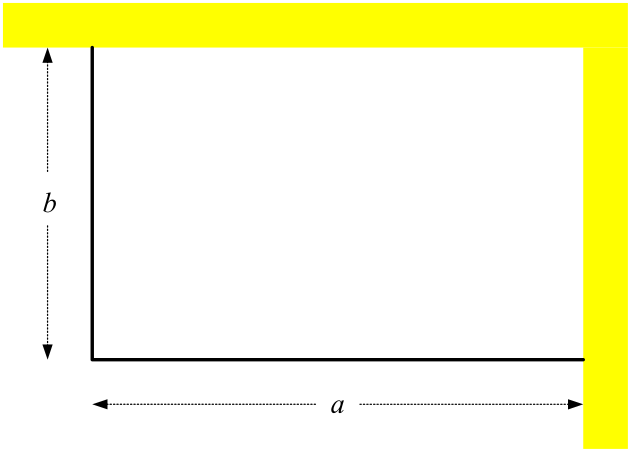
\includegraphics[ width=2.5711in, height=1.8498in,]{L4SZ2838}
}


\item A cylindrical can is to be made to hold $1\,$L of oil. Find the dimensions that will minimise the cost of the
metal to manufacture the can. (Hint: 1\thinspace L = $1000 cm^{3}$ 

\item Find the area of the greatest rectangle that can be inscribed in a semicircle
of radius $r$. 

\item If $1200 cm^{2}$ of material is available to make a box with a square base and an open top. Find the largest
possible volume of the box. (Hint: There is no wasted material.) \end{enumerate}


\subsection{Answers}
%TCIMACRO{\TeXButton{Start Two Columns}{\columnsep =30pt
% \begin {multicols}{2}}}%
%BeginExpansion
\columnsep =30pt
\begin {multicols}{2}
%EndExpansion
 \textbf{Exercises 5.1} 

1(a) $8$\qquad (b) $15$\qquad (c) $(2 a +h)$ 

2(a) $3$\qquad (b) $3$ \qquad (c) $3$ \\\relax (d) The average rate is always $3$ 

\textbf{Exercises 5.2.1} 

$y =2 x +3$ 

\textbf{Exercises 5.3} 

1. $23$\qquad 2. $ -12$\qquad 3. $4$\qquad 4. $\frac{1}{4}$ 

\textbf{Exercises 5.5.1} 

1(a) $f^{ \prime } (x) = -2 x^{ -3} =\frac{ -2}{x^{3}}$ 

1(b) $f^{ \prime } \left (x\right ) =\frac{2}{3} x^{ -\frac{1}{3}} =\frac{2}{3 \sqrt[{3}]{x}}$ 

2. Tangent line is $2 y -3 x +1 =0$ \\\relax Normal line is $3 y +2 x -5 =0$ 

Supplementary Exercises 

1. $y^{ \prime } =5 x^{4}$ 

2. $y^{ \prime } = -3 x^{ -4}$ 

3. $y^{ \prime } = -4 x^{ -5}$ 

4. $y^{ \prime } =\frac{3}{4} x^{ -\frac{1}{4}}$ 

5. $y^{ \prime } = -\frac{1}{2} x^{ -\frac{3}{2}}$ 

\textbf{Exercises 5.5.2} 

1(a) $12 x^{3}\text{\quad \quad }$1(b) $ -1$ 

\textbf{Exercises 5.5.3 and 5.5.4} 

1. $8 x^{7} +60 x^{4} -16 x^{3} +30 x^{2} -6$ 

2. $\left (0 ,4\right ) ,\text{\quad \quad }\left (\sqrt{3} , -5\right ) ,\text{\quad \quad }\left ( -\sqrt{3} , -5\right )$ 

Supplementary Exercises 

1(a) $2 x^{4}\text{\quad \quad }$(b) $0$\qquad (c) $ -12 x^{3}$ 

1(d) $ -8 x^{ -5} =\frac{ -8}{x^{5}}\text{\quad \quad }$(e) $ -x^{ -4} =\frac{ -1}{x^{4}}$ 

2(a) $\frac{1}{2} t^{ -\frac{1}{2}} =\frac{1}{2 \sqrt{t}}\text{\quad \quad }$(b) $\frac{3}{2} t^{\frac{1}{2}} =\frac{3 \sqrt{t}}{2}$ 

2(c) $\frac{5}{3} z^{\frac{2}{3}} =\frac{5 \sqrt[{3}]{z^{2}}}{3}\text{\quad \quad }$(d) $6.4 x^{2.2}$ 

3(a) $f^{ \prime } \left (x\right ) =6 x^{2} -6 x +4$ 

3(b) $f^{ \prime } \left (x\right ) =2 x +1 -\frac{1}{x^{2}}$ 

4. $\frac{d s}{d t} =8 t -7$ 

5. $\frac{d \left (3 x\right )}{d x} =3$ 

6. $\frac{d \left (3 u^{4}\right )}{d u} =12 u^{3}$ 

7. $D f \left (x\right ) =2$ 

\textbf{Exercises 5.6.2} 

1. $f^{ \prime } \left (x\right ) =e^{x} -1$ 

2. $\left (\ln  2 ,2\right ) \approx \left (0.69 ,2\right )$ 

Supplementary Exercises 

1. $a = -\frac{1}{3}$ or $ -1$ 

2. $f^{ \prime } \left (x\right ) =81 x^{2}$ 

3. $g^{ \prime } \left (x\right ) =15 x^{14}$ 

4. $f^{ \prime } \left (x\right ) =e^{x} -e x^{e -1}$ 

5. $x = \pm \sqrt{\frac{2}{3}}$ 

6. $f^{ \prime } \left (x\right ) = -3 x^{ -4} +\frac{3}{4} x^{ -1\frac{3}{4}} = -\frac{3}{x^{4}} +\frac{3}{4 \sqrt[{4}]{x^{7}}}$ 

7. $f^{ \prime } \left (x\right ) =\frac{1}{4} x^{ -\frac{3}{4}} +\frac{1}{12} x^{ -\frac{11}{12}} =\frac{1}{4 \sqrt[{4}]{x^{3}}} +\frac{1}{12 \sqrt[{12}]{x^{11}}}$ 

8. $g^{ \prime } \left (x\right ) =2 e x +2 e^{x} +e^{2} +e^{2} x^{e^{2} -1}$ 

9. $f^{ \prime } \left (x\right ) =\frac{1}{3} x^{ -\frac{2}{3}} =\frac{1}{3 \sqrt[{3}]{x^{2}}}$ 

\textbf{Exercises 5.7.1} 

1. $f^{ \prime } \left (x\right ) =x e^{x} +e^{x} =e^{x} \left (x +1\right )$ 

2 $g^{ \prime } \left (x\right ) =x^{2} e^{x} +2 x e^{x} =x e^{x} \left (x +2\right )$ 

3. $\frac{d y}{d r} =e^{r} \left (r^{2} -2\right )$ 

Supplementary Exercises 

1. $\left (x^{3} e^{x}\right )^{ \prime } =x^{3} e^{x} +3 x^{2} e^{x} =x^{2} e^{x} \left (x +3\right )$ 

2. $\left (x^{ -3} e^{x}\right )^{ \prime } =x^{ -3} e^{x} -3 x^{ -4} e^{x} =\frac{e^{x}}{x^{4}} \left (x -3\right )$ 

3.$\left (\left (x +1\right ) e^{x}\right )^{ \prime } =e^{x} \left (x +2\right )$ 

4. $\left (\left (x +2\right ) \left (x -2\right ) e^{x}\right )^{ \prime } =e^{x} \left (x^{2} +2 x -4\right )$ 

\textbf{Exercises 5.7.2} 

1. $y^{ \prime } =\frac{ -5}{\left (2 x -1\right )^{2}}$ 

2. $y^{ \prime } =\frac{x e^{x}}{\left (x +1\right )^{2}}$ 

3. $\frac{d f}{d t} =\frac{2 -2 t^{2}}{\left (1 +t^{2}\right )^{2}}$ 

4. $f^{ \prime } \left (x\right ) =\frac{ -A C e^{x}}{\left (B +C e^{x}\right )^{2}}$ 

Supplementary Exercises 

1. $\frac{ -3 x \left (x -2\right )}{\left (x -1\right )^{2}}$ 

2. $\frac{2}{\left (x +1\right )^{2}}$ 

3. $\frac{2 -x}{2 \sqrt{x} \left (x +2\right )^{2}}$ 

4. $\left (1 +x -2 x^{2}\right ) e^{ -x}$ 

\textbf{Exercises 5.7.3} 

1. Tangent $y =x$\qquad Normal $y = -x$ 

2. $2 y +x -2 =0$ 

3. Horizontal line $y =\frac{1}{2}$ 

\textbf{Exercises 5.8.1} 

1. $\left (f \circ g\right ) \left (x\right ) =\sqrt{x^{3}}\text{\quad \quad }\left (g \circ f\right ) \left (x\right ) =\left (\sqrt{x}\right )^{3}$ 

2. $\left (h \circ j\right ) \left (x\right ) =e^{\frac{x^{2}}{2}} =e^{x^{2}/2}\text{\quad \quad }\left (j \circ h\right ) \left (x\right ) =\frac{e^{2 x}}{2}$ 

\textbf{Exercises 5.8.5} 

1. $F^{ \prime } (x) =\frac{x}{\sqrt{1 +x^{2}}}$ 

2. $\frac{d y}{d x} = -10 x \left (1 +x^{2}\right )^{4}$ 

3. $\left (e^{x^{2}}\right )^{ \prime } =2 x e^{x^{2}}$ 

4. $\left (e^{e^{x}}\right )^{ \prime } =e^{e^{x}} \cdot e^{x} =e^{e^{x} +x}$ 

Supplementary Exercises 

1. $9 \left (3 x +2\right )^{2}$ 

2. $ -9 \left (4 -3 x\right )^{2}$ 

3. $\frac{3}{\left (5 x +3\right )^{2/5}}$ 

4. $\frac{ -2}{\left (2 x +1\right )^{2}}$ 

5. $\frac{9}{\left (4 -x\right )^{4}}$ 

6. $\frac{1}{\sqrt{2 x -5}}$ 

7. $\frac{ -2}{3 \sqrt[{3}]{\left (5 -x^{2}\right )^{2}}}$ 

8. $\frac{ -1}{2 \sqrt{\left (x +2\right )^{3}}}$ 

9. $6 x^{2} e^{2 x^{3}}$ 

\textbf{Exercises 5.9} 

1. $2 x e^{ -2 x} \left (1 -x\right )$ 

2. $ -e^{ -x} (1 -2 x) \left (5 -2 x\right )$ 

3. $\frac{1 -p}{\left (p^{2} +1\right ) \sqrt{p^{2} +1}}$ 

Supplementary Exercises 

1. $\left (x^{2} +3\right ) \left (5 x^{2} -16 x +3\right )$ 

2. $\left (x -3\right )^{2} \left (2 x -1\right )$ 

3. $\frac{\left (x -1\right ) \left (5 x +3\right )}{2 \sqrt{x +1}}$ 

4. $\frac{e^{x^{2}} \left (2 x +1\right )^{2}}{2 \sqrt{x +1}}$ 

5. $\frac{x -3}{\left (x +1\right )^{3}}$ 

6. $\frac{\left (x -3\right )^{2} \left (2 x +9\right )}{\left (x +2\right )^{2}}$ 

\textbf{Exercises 5.10.2} 

3. $x^{2} \cos  x +2 x \sin  x$ 

4. $\sqrt{x} \cos  x +\frac{1}{2 \sqrt{x}} \sin  x$ 

5. $5 \sec ^{2} 5 x$ 

6. $\frac{\cos  x +x \sin  x}{\cos ^{2} x}$ 

7. $ -\omega  \sin  \left (\omega  t +\delta \right )$ 

8. $y -x -1 =0$ 

9. $\frac{d x}{d \theta } =5 \mathrm{m}/\mbox{rad}$ 

Supplementary Exercises 

1. $4 \cos  4 x$ 

2. $2 \cos  \pi  x$ 

3. $5 \cos  \left (x +\frac{\pi }{4}\right )$ 

4. $ -15 \sin  3 x$ 

5. $36 \sin  \left (\frac{\pi }{2} -3 x\right )$ 

6. $3 \sec ^{2} 3 x$ 

7. $3 \sec ^{2} \left (x +2\right )$ 

8. $3 \sin ^{2} x \cos  x$ 

9. $6 \sin  3 x \cos  3 x$ 

10. $6 \left (x -1\right ) \sin ^{2} \left (x -1\right )^{2} \cos  \left (x -1\right )^{2}$ 

11. $4 \left (\pi  -x\right ) \cos  \left (\pi  -x\right )^{2} \sin  \left (\pi  -x\right )^{2}$ 

12. $4 \tan  2 x \sec ^{2} 2 x$ 

\textbf{Exercises 5.12.2} 

1. $\frac{d y}{d x} =\frac{1}{t}\text{,}$ Let $t =1\text{,}$ $y -x =0$ 

2. $y +x =\sqrt{2}\text{,}$ Horizontal when $t =\frac{\pi }{2}$ or $\frac{3 \pi }{2}\text{,}$ Vertical when $t =0$ or $\pi $ 

3. $2 y +4 \sqrt{3} x =6 +\sqrt{3}\text{,}$ Horizontal when $t =\frac{\pi }{4}\text{,}$ $\frac{3 \pi }{4}\text{,}$ $\frac{5 \pi }{4}\text{,}$ $\frac{7 \pi }{4}$ Vertical when $t =0\text{,}$ $\pi $ 

Supplementary Exercises 

1. $\frac{t \left (3 t^{2} +1\right )}{2 t +1}$ 

2. $\frac{\cos  t +\sin  t}{\cos  t -\sin  t}$ 

3. $\frac{1}{t}$ 

4. $ -\frac{b}{a} \tan  \theta $ 

5. $ -2 \sin  \theta $ because $\sin  2 \theta  =2 \sin  \theta  \cos  \theta $ 

6. $\frac{\sin  \theta }{1 -\cos  \theta }$ 

\textbf{Exercises 5.13} 

1. $3 y +4 x -25 =0$ 

2. $y +x +1 =0$ 

3(a) $\frac{4 x}{9 y}$ 

3(b) $\frac{x \left (8 -x^{2} -y^{2}\right )}{y \left (8 +x^{2} +y^{2}\right )}$ 

3(c) $\frac{y e^{x}}{3 y^{2} -e^{x}}$ 

Supplementary Execises 

1. $ -\frac{1}{2 y}$ 

2. $ -\frac{x}{y}$ 

3. $ -\frac{x}{3 y}$ 

4. $ -\frac{1 +y}{x}$ 

5. $\frac{1 -y}{x}$ 

6. $ -\frac{y}{x}$ 

7. $\frac{2 x +y}{1 -x}$ 

8. $ -\frac{x +2 y}{2 x +y}$ 

\textbf{Exercises 5.14} 

1. $\frac{1}{x}$ 

2. $\frac{2 x}{x^{2} +1}$ 

3. $\frac{1}{\tan  x}$ 

4. $\frac{1}{x}$ 

Supplementary Exercises 

1. $\frac{1}{x}$ 

2. $\frac{1}{x -5}$ 

3. $\frac{1}{2 \left (x +2\right )}$ 

4. $\frac{3}{x +2}$ 

5. $\frac{1}{x} +\frac{1}{x +2} -\frac{1}{x +1} =\frac{x^{2} +2 x +2}{x \left (x +1\right ) \left (x +2\right )}$ 

6. $\frac{1}{2} \left (\frac{1}{x +1} -\frac{ -1}{1 -x}\right ) =\frac{1}{\left (x +1\right ) \left (1 -x\right )}$ 

\textbf{Exercises 5.15.1} 

1. $3 x^{2} \frac{d x}{d t}$ 

2. $\frac{d A}{d t} =48 cm^{2}/\mbox{s}$ 

3. $\frac{d A}{d t} =60 \pi  \mathrm{m}/\mbox{s}$ 

4. $ -\frac{1}{20 \pi }$ \\\relax decreasing at a rate of $\frac{1}{20 \pi } cm/\mbox{min}$ 

5. $\frac{215}{\sqrt{101}} \approx 21.4 \mathrm{m}/\mbox{h}$ 

6. $\frac{800 \sqrt{5}}{3} \approx 596.3 km/\mbox{h}$ 

\textbf{Exercises 5.15.2} 

1. The two parts are $25$ and $25$ 

2. The number is $\frac{1}{2}$ 

3. Dimensions are $1200 \mbox{m}$ by $600 \mbox{m}$ 

4. Dimensions are $150 \mbox{m}$ by $150 \mbox{m}$ 

5. $r =\sqrt[{3}]{\frac{500}{\pi }} \approx 5.4 \mbox{cm}\text{,}$ and $h =2 r$ 

6. Area $ =r^{2}$ 

7. Dimensions are 20 by 20 by 10, \\\relax Volume $ =4000 cm^{3}$ 


\end {multicols}

